% \iffalse
\let\negmedspace\undefined
\let\negthickspace\undefined
\documentclass[journal,12pt,twocolumn]{IEEEtran}
\usepackage{cite}
\usepackage{amsmath,amssymb,amsfonts,amsthm}
\usepackage{algorithmic}
\usepackage{graphicx}
\usepackage{textcomp}
\usepackage{xcolor}
\usepackage{txfonts}
\usepackage{listings}
\usepackage{enumitem}
\usepackage{mathtools}
\usepackage{gensymb}
\usepackage{comment}
\usepackage[breaklinks=true]{hyperref}
\usepackage{tkz-euclide} 
\usepackage{listings}
\usepackage{gvv}                                        
\def\inputGnumericTable{}                                 
\usepackage[latin1]{inputenc}                                
\usepackage{color}                                            
\usepackage{array}                                            
\usepackage{longtable}                              
\usepackage{calc}                                             
\usepackage{multirow}                                         
\usepackage{hhline}                                           
\usepackage{ifthen}                                           
\usepackage{lscape}

\newtheorem{theorem}{Theorem}[section]
\newtheorem{problem}{Problem}
\newtheorem{proposition}{Proposition}[section]
\newtheorem{lemma}{Lemma}[section]
\newtheorem{corollary}[theorem]{Corollary}
\newtheorem{example}{Example}[section]
\newtheorem{definition}[problem]{Definition}
\newcommand{\BEQA}{\begin{eqnarray}}
\newcommand{\EEQA}{\end{eqnarray}}
\newcommand{\define}{\stackrel{\triangle}{=}}
\theoremstyle{remark}
\newtheorem{rem}{Remark}
\begin{document}

\bibliographystyle{IEEEtran}
\vspace{3cm}

\title{NCERT DISCRETE}
\author{EE23BTECH11020 - Raghava Ganji$^{*}$% <-this % stops a space
}
\maketitle
\newpage
\bigskip

\renewcommand{\thefigure}{\theenumi}
\renewcommand{\thetable}{\theenumi}
\textbf{Question 11.9.4.3:}
Find the sum to n terms to the series $3\brak 1^2+5\brak 2^2+7\brak 3^2+ \ldots$\\ 
\solution\\
Given series is $3\brak 1^2+5\brak 2^2+7\brak 3^2+ \ldots$\\\\
\begin{table}[h]
\centering
\begin{tabular}{|c|c|c|}\hline
$x\brak 0$ & $3$ & 1st\hspace{1mm}term\\ \hline
$x\brak n$ & $?$ & \brak {n+1}th\hspace{1mm}term\\ \hline
$y\brak {n-1}$ & $?$ & sum\hspace{1mm}of\hspace{1mm}n\hspace{1mm}terms\\ \hline
\end{tabular}
\caption{parameters}
\end{table}

\begin{align}
x\brak n&=\brak{2n+3}\brak{n+1}^2\\
y\brak n&=x\brak n*u\brak n\\
Y\brak z&=X\brak zU\brak z\\
X\brak z&=\frac{3+8z^{-1}+z^{-2}}{\brak{1-z^{-1}}^4}\\
U\brak z&=\frac{1}{1-z^{-1}}\\
\implies Y\brak z&=\frac{3+8z^{-1}+z^{-2}}{\brak{1-z^{-1}}^5}
\end{align}
Using\eqref{}
\begin{align}
y\brak n&=\frac{1}{2\pi j}\oint_C\frac{\brak{3+8z^{-1}+z^{-2}}z^{n-1}}{\brak{1-z^{-1}}^5}dz\nonumber  \\
y\brak n&=\lim_{z\to 1}\frac{1}{4!}\frac{d^4}{dz^4}\frac{3z^{n-1}+8z^{n-2}+z^{n-3}}{\brak{1-z^{-1}}^5}\brak {1-z^{-1}}^5\\
\implies y\brak n&=\frac{\brak{n+1}\brak{n+2}\brak{3n^2+11n+9}}{6}\\
\implies y\brak {n-1}&=\frac{n\brak{n+1}\brak{3n^2+5n+1}}{6}
\end{align}
\begin{figure}
    \centering
    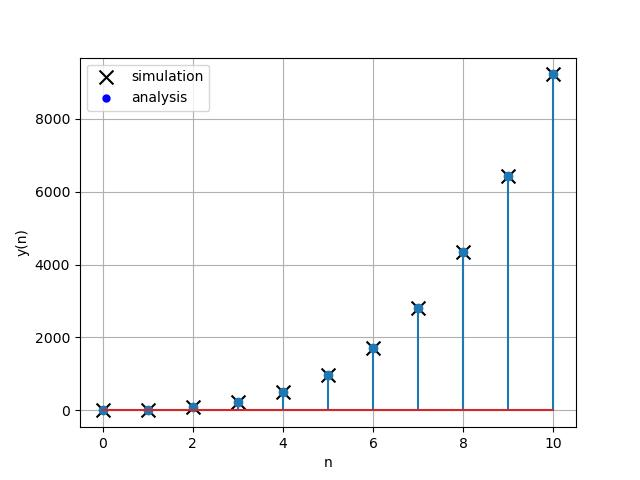
\includegraphics[width=1\columnwidth]{11.9.4.3.1.jpg}
    \caption{simulation vs analysis of y\brak n}
\end{figure}
\end{document}
